\section{Evaluations and Discussion}




\subsection{Overhead}




In this section we will measure the latency introduced in the application to record a heartbeat

\subsubsection*{Methodology}



overhead

\subsection{Application}

Andy

\subsection{Experiments}

We will go over three different experiments to evaluate Anchors.

\subsubsection{Experiment 1: Monitor across Different Scheduler}
\hfill \linebreak
In this experiments, we want to evaluate Anchors' ability to monitor and save CPU resource when VMs are running on different subset of cores with different scheduler.

\begin{itemize} 
\item[--] VM Configuration: \\
Anchors requires the hypersvisor scheduler to be able to assign specific amount of CPU resource to the VMs. With one VM, under RTDS Scheduler, the amount CPU resource allocated to the VM can be specified by assigning proper period and budget. But for Credit Scheduler, which allocates CPU resource based on weights, it is required to create a dummy VM under the same CPU pool so precise CPU resource allocation can be achieved by assigning proper weights to the dummy and the main VM. To have a fair comparison, we also create a dummy VM for the CPU pool that runs RTDS Scheduler. Both dummy were assigned 1\% of the CPU utilization before every trial.
The complete VM configuration are shown in table \ref{exp1vmsetup}

\begin{table}[ht]
\centering
\caption{My caption}
\label{exp1vmsetup}
\begin{tabular}{@{}cccc@{}}
\toprule
\textbf{}                     & \textbf{\# of VCPUs}     & \textbf{Scheduler}          & \textbf{\begin{tabular}[c]{@{}c@{}}Initial CPU\\ Utilization\end{tabular}} \\ \midrule
\rowcolor[HTML]{EFEFEF} 
{\color[HTML]{333333} VM1}    & {\color[HTML]{333333} 5} & {\color[HTML]{333333} RTDS} & {\color[HTML]{333333} 99\%}                                                \\
\rowcolor[HTML]{EFEFEF} 
{\color[HTML]{333333} Dummy1} & {\color[HTML]{333333} 5} & {\color[HTML]{333333} RTDS} & {\color[HTML]{333333} 1\%}                                                 \\
\rowcolor[HTML]{C0C0C0} 
VM2                           & 5                        & Credit                      & 99\%                                                                       \\
\rowcolor[HTML]{C0C0C0} 
Dummy2                        & 5                        & Credit                      & 1\%                                                                        \\ \bottomrule
\end{tabular}
\end{table}



\item[--] Application:\\
In this experiment, we run the object detection application for on both VM1 and VM2. The duration of each trial is 120 seconds, the first 40 seconds are running under high workload mode, between 40-80 seconds the workload is switched to light, and finally between 80-120 seconds the workload is switched medium, as shown in figure meow. 


\item[--] Methodology:\\
For each scheduler, three different controllers, static, AIMD and APID are applied. The CPU utilization and FPS data are collected for analysis.

\item[--] Result:\\
hi
\end{itemize}





\subsubsection{Experiment 2: Monitor across Multiple VMs}

\hfill \linebreak
In this experiment, we use Anchors to monitor VM1 and VM2 that are running on the same set of PCPU with RTDS scheduler, and shows VM3 is able to benefit from the saved CPU utilization.


\begin{itemize} 

\item[--] VM Configuration:\\
There are three VMs fo this experiment 

\item[--] Application:\\
\item[--] Methodology:\\
\item[--] Result:\\

\end{itemize}
\subsection*{Experiment 3: Monitor under Overloading System}


\hfill \linebreak
In this experiment, we show that Anchors is able to improve the overall real-time performance when the system is not able to provide enough CPU resource to satisfy the total demand from VMs.


\begin{itemize} 

\item[--] VM Configuration:\\
\item[--] Application:\\
\item[--] Methodology:\\
\item[--] Result:\\

\end{itemize}



\iffalse
\section{Results and Discussion}
\label{s4}

\subsection{Experiment Setup}

Our simulation adopts the system with seven local fog servers as illustrated in Figure \ref{car7} and an additional cloud server. For fog servers, the link rate between server $i$ and server $j$, $B_{ij}$, is randomly drawn from between 16 and 64 tasks per second for $i\ne j$, or $\infty$ for $i=j$, the CPU frequency for server $j$, ${f_{j}}$, is randomly drawn from between 2700 MHz and 3600 MHz, and the capacity of server $j$, $C_{j}$,  is randomly drawn from between 10 and 35 tasks. For the remote cloud server, its initial tasks, $N_{cloud}$ is 0, $B_{icloud}$ is 4 tasks per second, ${f_{cloud}}$ is 4500MHz, and $C_{cloud}$ is $\infty$. For all servers, CPU cycles required per task, $x$, is set at 35 Mcycles, deadline for each task, $D$, is set at 0.5 second, and allowed processing time for each server, $\tau$, is 0.48 second. The system's parameters can be summarized in Table \ref{simvar}.

A taskset is generated by randomly selecting a number for $N_{i}$ from a range of integers which is shown in the first row in Table \ref{ntypes}. By varying the range of integers for $N_{i}$, we can create different loadings for the system. In each experiment, for the same type of loading, taskset generation is performed 100 times, and load balancing optimization is executed for each newly generated taskset. We record all the $N_{i}$ values and so each experiment can be run with the same tasksets. All the experiments were run in the machine with dual quadcore AMD Opteron 2.3 GHz with 16GB memory. The time it takes to execute linear prediction and to solve the optimization on that machine are both less than 0.01 second for all the experiments we run. So the overhead for mobility prediction and load balancing is less than 0.02 second, which is within the overhead budget, calculated by substracting deadline by allowed processing time, $D-\tau=0.5-0.48=0.02$.


\begin{table}[ht!]
\caption{Simulation Parameters}
\centering
\small
\begin{tabular}{| m{0.8cm} | m{1.6cm} | m{15em} |}
    \hline
    \multicolumn{3}{|l|}{\textbf{Simulation Parameters for the System}}\\
    \hline
    $k$ & 8 & Number of servers \\
    \hline
    $x$ & 35 & Number of CPU cycles required for each task (Mcycles)\\
    \hline
    $D$ & 0.5 & Deadline for all tasks (sec)\\
    \hline
    $\tau$ & 0.48 & Allowed processing time for each server (sec)\\
    \hline
    \multicolumn{3}{|l|}{\textbf{Simulation Parameters for Local Fog Servers}}\\
    \hline
    $N_{i}$ & see Table \ref{ntypes} & Number of initial tasks for server $i$\\
    \hline
    \multirow{2}{*}{$B_{ij}$} & [16,64] & Link rate between server $i$ and server $j$ for $i\ne j$ (tasks/sec) \\ \cline{2-3}
    & $\infty$ & Link rate between server $i$ and server $j$ for $i=j$ (tasks/sec) \\
    % $B_{ij}$ & [16,64] & Link rate between server $i$ and server $j$ (tasks/sec)\\
    \hline
    $C_{j}$ & [10,35] & Capacity of server $j$ (tasks)\\
    \hline
    $f_{j}$ & [2700,3600] & CPU frequency of server $j$ (MHz)\\
    \hline
    \multicolumn{3}{|l|}{\textbf{Simulation Parameters for Cloud Server}}\\
    \hline
    $N_{cloud}$ & 0 & Number of inital tasks for cloud server\\
    \hline
    $B_{icloud}$ & 4 & Link rate between server $i$ and cloud server (tasks/sec)\\
    \hline
    $C_{cloud}$ & $\infty$ & Capacity of cloud server (tasks)\\
    \hline
    $f_{cloud}$ & 4500 & CPU frequency of cloud server (MHz)\\
    \hline\hline
    \multicolumn{2}{|l|}{\textbf{Optimizing Variables}}\\
    \hline
    $n_{ij}$ & solved with optimization & Number of tasks distributed from server $i$ to server $j$\\
    \hline
\end{tabular}
\label{simvar}
\end{table}

\begin{table}[h]
\caption{Types of Workloads}
\small
\centering
\begin{tabular}{|m{1cm}|m{1cm}|m{1cm}|m{1cm}|m{1cm}|m{1cm}|}
    \hline
    Range for $N_{i}$ (tasks)& [10,26] & [10,28] & [10,30] & [10,32] & [10,34] \\ \hline
    Total number of tasks & 12687 & 13472 & 14143 & 14739 & 15051 \\ \hline
\end{tabular}
\label{ntypes}
\end{table}

\subsection{Deadline Misses vs Total Runtime}

In this experiment, we focus on the varying $v$, the weighing parameter in the optimization formulation presented. According to our objective function (\ref{opt_fstart}), a greater $v$ value should result in fewer deadline misses with higher total runtime. We verify such trend by running experiment with different $v$ and gather the results for deadline misses and total runtime respectively, as shown in Figure \ref{res_opt_vs_opt_md} and Figure \ref{res_opt_vs_opt_time}. From the figures, we observe that a larger $v$ does result in fewer deadline misses and higher total runtime.


\begin{figure}[h!]
\centering
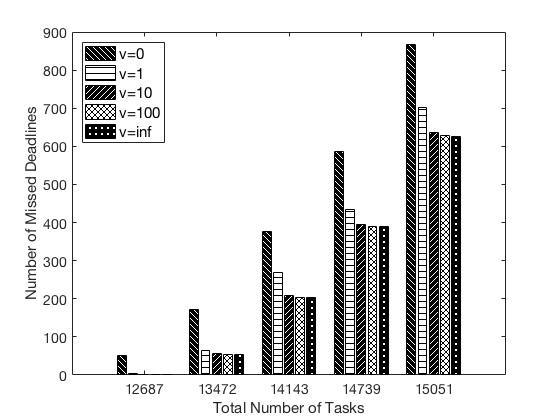
\includegraphics[width=1\linewidth]{images/res_opt_vs_opt_mdp}
\caption{Deadline Misses Comparison with Different $v$ }
\label{res_opt_vs_opt_md}
\end{figure}


\begin{figure}[h!]
\centering
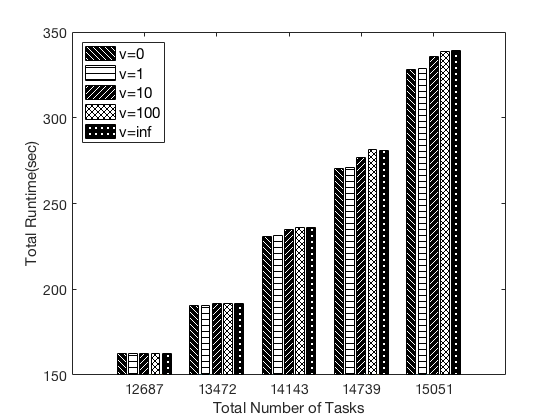
\includegraphics[width=1\linewidth]{images/res_opt_vs_opt_timep}
\caption{Total Runtime Comparison with Different $v$ }
\label{res_opt_vs_opt_time}
\end{figure}


\subsection{Comparison with Other Load Balancing Algorithms}



We compare our optimization result with local static, a simple load balancing method, and three other commonly used load balancing algorithms: weighted round robin, active monitoring and throttled load balancer\cite{wrr}\cite{amt}\cite{amt2}. In local static load balancing, each server with initial tasks exceed its capacity will transfer all the overloading tasks to the cloud server. Weighted round robin is implemented by assigning high weights for local servers that have not reached their maximum capacity. The cloud server will have a higher weight than a local server only when that server reaches its maximum capacity. Active monitoring load balancing is implemented by having each task assigned to the local server that has the highest remaining capacity, the algorithm will only assign to the cloud server when all the local servers are full. In the throttled load balancer, each task is assigned based on the most suitable server available, so the server with lowest completion time and has not reached its maximum capacity will be assigned with the new task. Again, a cloud server will be utilized only when none of the local servers are available. The comparisons are shown in Figure \ref{res_opt_vs_lb_ls_md} and Figure \ref{res_opt_vs_lb_ls_time}. Local static does not utilize any available local server so it is not surprising that local static is outperformed by more than 50\% in every case. On the other hand, our optimization has the least deadline misses and total runtime for every case. The numerical results for deadline misses is presented in Table \ref{good}. From Table \ref{good}, at a lighter load of 13472 tasks, our optimization outperforms throttled load balancer which has the second least deadline misses, by almost 50\%, but as the load of the system increases, the improvement brought by optimization starts to decrease. At the heaviest load of 15051 tasks, the improvment our optimization can bring drops to about 25\%. The reason being a heavy loaded system has fewer available options for task distributing, thus the potential for a better performance gets smaller as more load is added to the system.




 
% \begin{figure}[ht!]
% \centering
% 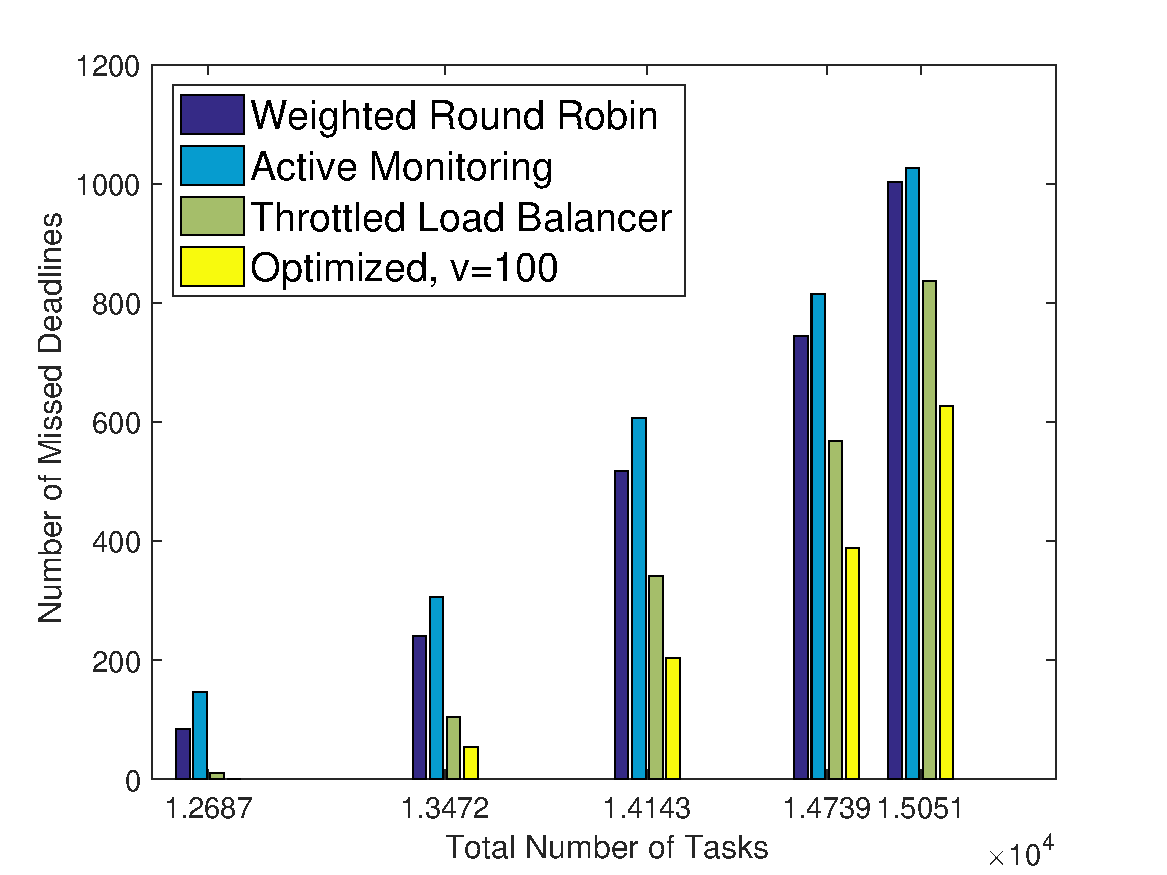
\includegraphics[width=1\linewidth]{images/res_opt_vs_lb_md}
% \caption{Deadline Misses Comparison with Other Load Balancing Algorithms}
% \label{res_opt_vs_lb_md}
% \end{figure}


% \begin{figure}[ht!]
% \centering
% 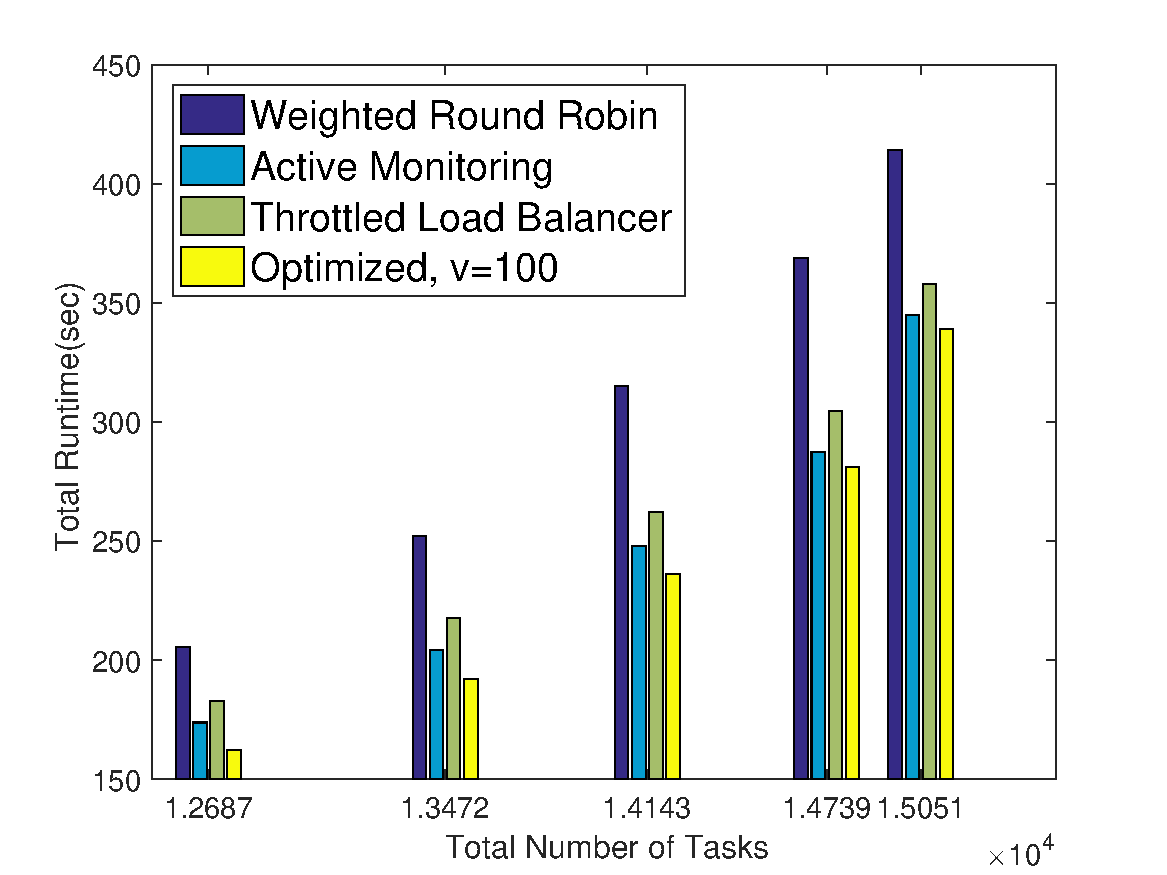
\includegraphics[width=1\linewidth]{images/res_opt_vs_lb_time}
% \caption{Total Runtime Comparison with Other Load Balancing Algorithms}
% \label{res_opt_vs_lb_time}
% \end{figure}

 
\begin{figure}[ht!]
\centering
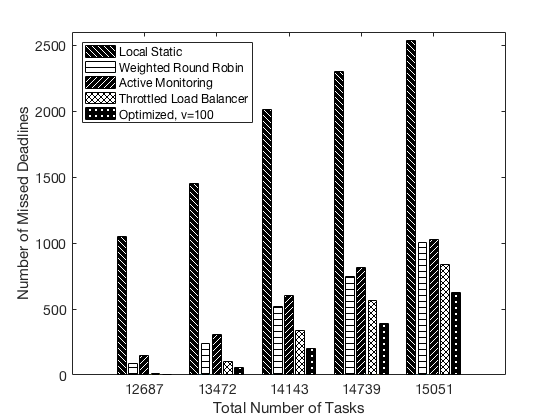
\includegraphics[width=1\linewidth]{images/res_opt_vs_lb_ls_mdp}
\caption{Deadline Misses Comparison with Other Load Balancing Algorithms}
\label{res_opt_vs_lb_ls_md}
\end{figure}


\begin{figure}[ht!]
\centering
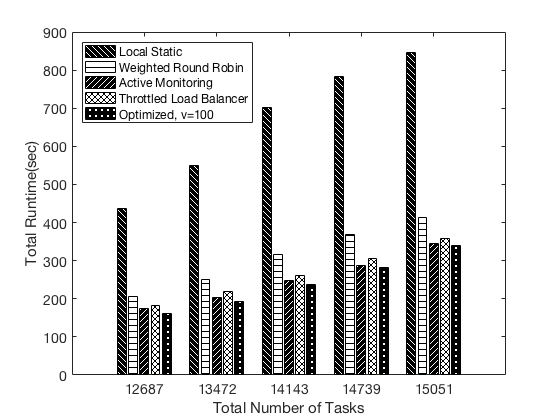
\includegraphics[width=1\linewidth]{images/res_opt_vs_lb_ls_timep}
\caption{Total Runtime Comparison with Other Load Balancing Algorithms}
\label{res_opt_vs_lb_ls_time}
\end{figure}

\begin{table}[h]
\small
\caption{Missed Deadlines Counts}
\centering
\begin{tabular}{|m{1.5cm}|m{0.75cm}|m{0.75cm}|m{0.75cm}|m{0.75cm}|m{0.75cm}|}
    \hline
    \textbf{Total number of tasks} & \textbf{12687} & \textbf{13472} & \textbf{14143} & \textbf{14739} & \textbf{15051} \\ 
    \hline
    Optimized, $v$=100 & 0 & 54 & 204 & 389 & 627 \\
    \hline
    Local Static & 1052 & 1454 & 2011 & 2300 & 2535 \\
    \hline
    Weighted Round Robin & 85 & 240 & 517 & 745& 1003 \\
    \hline
    Active Monitoring & 147 & 306 & 606 & 815& 1026 \\
    \hline
    Throttled Load Balancer & 11 & 104 & 341 & 568& 837 \\
    \hline
\end{tabular}
\label{good}
\end{table}

% \begin{table}[h]
% \small
% \caption{Missed Deadlines Counts}
% \centering
% \begin{tabular}{|m{1.5cm}|m{0.75cm}|m{0.75cm}|m{0.75cm}|m{0.75cm}|m{0.75cm}|}
%     \hline
%     \textbf{Total number of tasks} & \textbf{12687} & \textbf{13472} & \textbf{14143} & \textbf{14739} & \textbf{15051} \\ 
%     \hline
%     Optimized, $v$=100 & 0 & 54 & 204 & 389 & 627 \\
%     \hline
%     Local Static & 1052 & 1454 & 2011 & 2300 & 2535 \\
%     \hline
%     Weighted Round Robin & 85 & 240 & 517 & 745& 1003 \\
%     \hline
%     Active Monitoring & 147 & 306 & 606 & 815& 1026 \\
%     \hline
%     Throttled Load Balancer & 11 & 104 & 341 & 568& 837 \\
%     \hline
% \end{tabular}
% \label{good}
% \end{table}


% \begin{table}[h]
% \small
% \caption{Deadline Misses ratio - deadline misses/total tasks, $v$=100}
% \centering
% \begin{tabular}{|m{1.5cm}|m{0.75cm}|m{0.75cm}|m{0.75cm}|m{0.75cm}|m{0.75cm}|}
%     \hline
%     \textbf{Total number of tasks} & \textbf{12687} & \textbf{13472} & \textbf{14143} & \textbf{14739} & \textbf{15051} \\  
%     \hline
%     Optimized, $v$=100 & 0\% & .40\% & 1.44\% & 2.64\% & 4.17\% \\
%     \hline
%     Local Static & 8.29\% & 10.79\% & 14.2\% & 15.6\% & 16.8\% \\
%     \hline
%     Weighted Roung Robin & 0.67\% & 1.78\% & 3.66\% & 5.05\% & 6.66\% \\
%     \hline
%     Active Monitoring  & 1.16\% & 2.27\% & 4.28\% & 5.53\% & 6.82\% \\    
%     \hline
%     Thorttled Load Balancer & 0.087\% & 0.77\% & 2.41\% & 3.85\% & 5.56\% \\
%     \hline
% \end{tabular}
% \label{bad}
% \end{table}



% \begin{table}[h]
% \small
% \caption{Deadline Misses Comparison to Optimized \%, $v$=100}
% \centering
% \begin{tabular}{|m{1.5cm}|m{0.75cm}|m{0.75cm}|m{0.75cm}|m{0.75cm}|m{0.75cm}|}
%     \hline
%     \textbf{Total number of tasks} & \textbf{12687} & \textbf{13472} & \textbf{14143} & \textbf{14739} & \textbf{15051} \\ 
%     \hline
%     Local Static & 100\% & 96.3\% & 89.9\% & 83.1\% & 75.3\% \\
%     \hline
%     Weighted Roung Robin  & 100\% & 77.5\% & 60.5\% & 48.8\%& 37.5\% \\
%     \hline
%     Active Monitoring  & 100\% & 82.4\% & 66.3\% & 52.3\%& 38.9\% \\
%     \hline
%     Thorttled Load Balancer & 100\% & 48.1\% & 40.2\% & 31.5\%& 25.1\% \\
%     \hline
% \end{tabular}
% \label{best}
% \end{table}



\fi












